\Chapter{Alkalmazásbeli példa}

\Section{A kód}
\SubSection{Alapkoncepció}
Először egy egyszerű Python applikációba szerettem volna megvalósítani a megjelenítést és magát az egész projektet. Ehhez a TKInter nevű könyvtárat szándékoztam használni, állítható értékekkel, hogy megfigyeljem melyik érték kombinációval a legcélszerűbb a kép beolvasása és az adatok kinyerése onnan. Leegyszerűsített használatra, csak akkordokkal foglalkozva a kék színnel ábrázolt akkordokat szándékoztam kinyerni a képből. Végül a csúszkákat félretéve manuálisan írtam át az értékeket, egy numpy tömbbe csomagoltam be ezeket. Ezek az értékek kellettek ahhoz, hogy meghatározzam a cv2-nek, hogy milyen színskálába szeretném kiszedni az akkordokat. 
\par
Kísérleteztem azzal, hogy ha változtatom a skálát, akkor milyen pontossággal tudja visszaadni csak az akkordokat(amik kékkel vannak feltüntetve) a képről. Az volt a terv, hogy akkor ez mint bemeneti kép lesz majd kiolvasva a képből az OCR segítségével. Ehhez az kellett, hogy a megfelelő spektrumba legyen a program színhatára, amit ki tud olvasni zajmentesen, mivel a kották egységes kék színnel vannak kezelve akkordok terén, ezért nem kell egyáltalán változó értékű tömböket használni a színskála beállításához.
\par

\SubSection{Kimeneti példák}
A következőkben áttértem jupyter-notebookra, hogy lehessen szétbontani, és emészthetőbbé kialakítani a kódot.

\begin{python}
this_img = cv2.imdecode(numpyarray, cv2.IMREAD_UNCHANGED)	
\end{python}

\begin{figure}[h]
	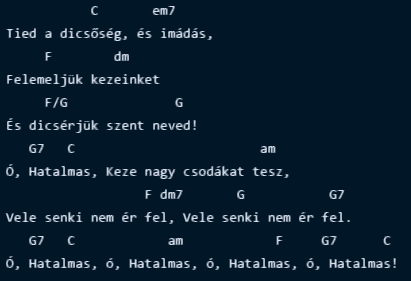
\includegraphics[scale=1]{images/output_tied.png}
	\caption{Az xml beolvasó program kimenete}
	\label{fig:output1}
\end{figure}

\begin{figure}[h]
	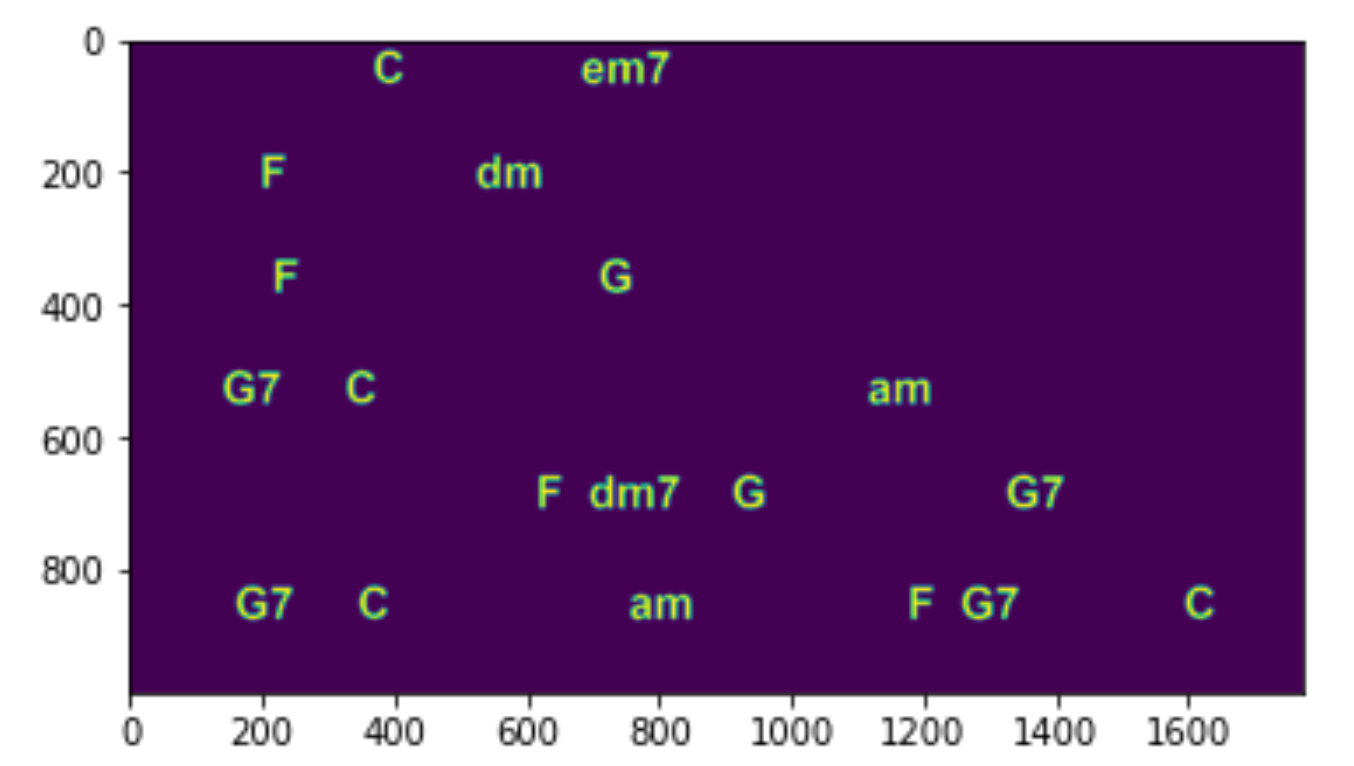
\includegraphics[scale=0.5]{images/output_justchords.png}
	\caption{Kotta akkordjai}
	\label{fig:output2}
\end{figure}

\begin{figure}[h]
	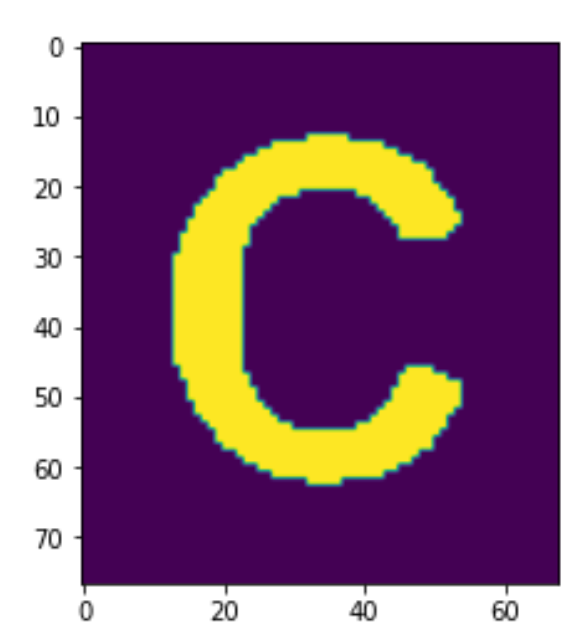
\includegraphics[scale=0.5]{images/output_single_character.png}
	\caption{A kotta egyik akkordja}
	\label{fig:output3}
\end{figure}

\Section{Tesseract használata}
A tesseract nevezetű OCR szoftvert használom a karakterfelismerésre a dolgozatban, nevezetesen a pytesseract függvénykönyvtárat. Ez alapvetően a Google OCR motorja, amit implementáltak python környezetben. Önmagába álló szkriptként is használható, és széles körben felismer különböző kiterjesztésű képeket, mint például a jpeg, png, gif, bmp, tiff és egyéb másokat, habár ugyanúgy megvannak a korlátai is, amiről majd később térek ki részletesebben. Elsőként mivel hogy különálló maga a program ezért PATH-ba kellett helyezni, amivel sajnos meggyűlt a baj, mivel hogy nem ismerte fel az operációs rendszer. Így a következőképpen oldottam meg, hogy használható legyen:
\begin{python}
	import pytesseract
	
	local_path =  r'C:\Program Files\Tesseract-OCR\tesseract.exe'
	pytesseract.pytesseract.tesseract_cmd = local_path
\end{python}
A lokális környezetbe való fejlesztés erejéig volt használatba ez az elérési útvonal. A függvénykönyvtárnak az image to string nevű metódusát használtam arra, hogy a képből szöveg váljon. Paraméterként megadható, hogy ugye mely képekből kell a szöveget kiolvasni, és többek között, amit használtam én is az a nyelv megadása, valamint konfigurációt is meg tudtam adni. A pontosság az elején zavaró volt, mert túlságosan zajos volt a kép sokszor, ahhoz, hogy az OCR megfelelően ki tudja venni, hogy mely karakterről is van szó. Ehhez az egyik megolás az volt, hogy jobban lehessen manipulálni a bemeneti képet, amivel dolgozik a Tesseract.